% section 3

\section{環境識別子による型システムの構築}

\subsection{先行研究のアイディア}

Tahaら\cite{Taha:2003:EC:604131.604134}は、純粋な(副作用のない)コード生成の言語の型安全性を保証するため、
環境識別子(Environment Classifier)を導入した。
環境識別子$\alpha$は、コード生成のステージに対応し、
「そのステージで使える(コードレベル)の変数とその型の集合(あるいは型文脈)」を抽象的に表現した変
数であり、$\codeT{\intT}{\alpha}$のように、コード型の一部として使用される。

須藤ら\cite{Sudo2014}は、破壊的変数を持つコード生成言語に対する型安全性を保証するため、
環境識別子を精密化した。本節では、須藤らのアイディアを解説する。
以下の図は、彼らの言語における危険なプログラム例である。
\begin{center}
  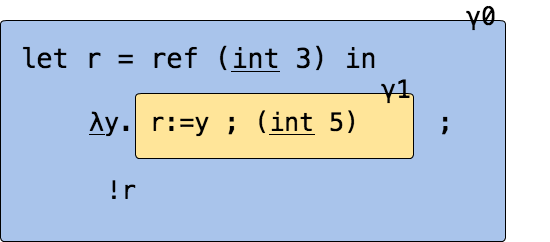
\includegraphics[clip,width=4cm]{./img/sudo_ref.png} 
  須藤らの「危険な」例
\end{center}
ここで、$r$は、整数のコードを格納する参照(破壊的セル)であり、$r:=y$と
$!r$はそれぞれ、$r$への代入と$r$の中身の読み出しを表す。
上記のプログラムは、コードレベルのラムダ抽象($y$に対するラムダ抽象)で
生成されるコードレベル変数を$u$とするとき、$\code{u}$を$r$に格納し、
$u$のスコープ(黄色で示したもの)が終わったあとに取り出しているため、
計算結果は、自由変数をもつコード$\code{u}$となり、危険である。

上記のようなプログラムを型エラーとするため、須藤らは、コードレベル変数の
スコープごとに環境識別子を割り当てた。
上記では外側のスコープ(青)が$\gamma_0$、
内側のスコープ(黄)が$\gamma_1$という環境識別子で表現される。
$\gamma_0$で有効なコードレベル変数はなく、
$\gamma_1$で有効なコードレベル変数は$y$(に対応して生成される変数)である。
$\gamma_0$のスコープは$\gamma_1$のスコープを含む。言い換えれば、
$\gamma_1$で使える変数の方が$\gamma_0$で使える変数の方が(同じか)多い。
このことを$\gamma_1 \ord \gamma_0$ と表すことにする。
$r$は $\codeT{\intT}{\gamma_0}$型を持つ。
$y$は $\gamma_1$で使える変数であるが、$\gamma_0$では使えないため、
$r$に$y$を代入することはできず、$r:=y$のところで型エラーとなる。

コードレベルの変数スコープと,型によるスコープの表現をあらわしたのが,以下の図である.
forやletなどコードレベルの束縛子があるたびに、新しいスコープが開かれ、
使える変数が増えていくことが分かるだろう.
\begin{center}
  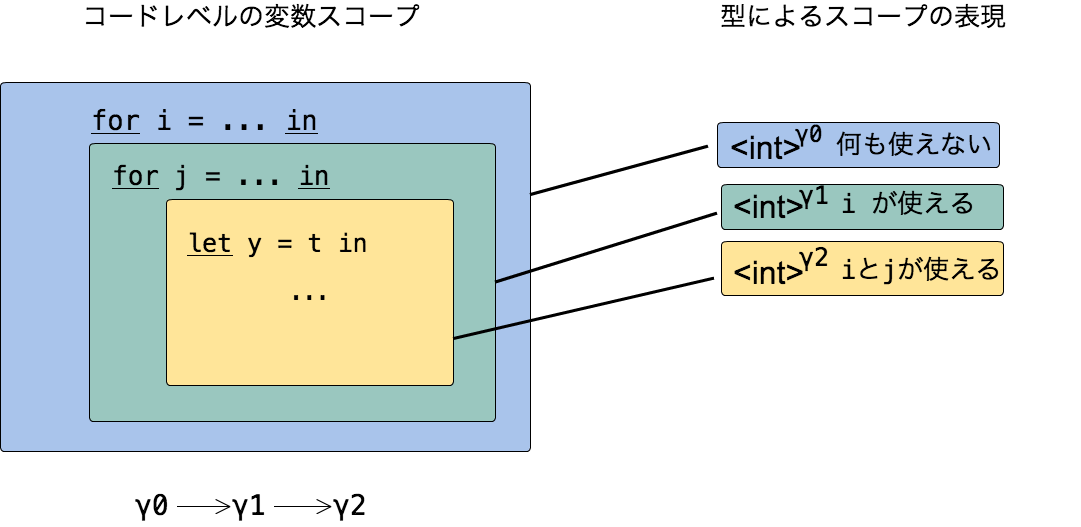
\includegraphics[clip,height=4cm]{./img/ec_for.png}
\end{center}

コードレベルの変数の型に、(精密化した)環境識別子を付与することで、その
変数が使えるスコープがわかり、破壊的代入などの副作用があるプログラムにおいても
スコープや型の安全性を保つことができる。

なお、須藤らの対象としていた言語が持っていた計算エフェクトは、「局所的なスコープをもつ参照」
であり、現実のOCaml/MetaOCaml等とは異なるものであった。
同一の著者グループは、最近、精密化した環境識別子のアイディアを用いて、
グローバルな参照を持つ言語に対するある種の型安全性
が成立することを示している\cite{Aplas2016}。

\subsection{本研究: 環境識別子の拡張}

本研究で扱う shift0/reset0によるコントロールエフェクトは、
須藤らによる精密化された環境識別子でも扱うことができない。本節では、そ
の問題点を明らかにし、その問題の解決の鍵となる join ($\cup$)の導入につ
いて述べる。

このため、前述の2重のforループ生成において、その中間にlet挿入をするプログラムに
ついて考察する。その概形は下記の左図である。
\begin{center}
  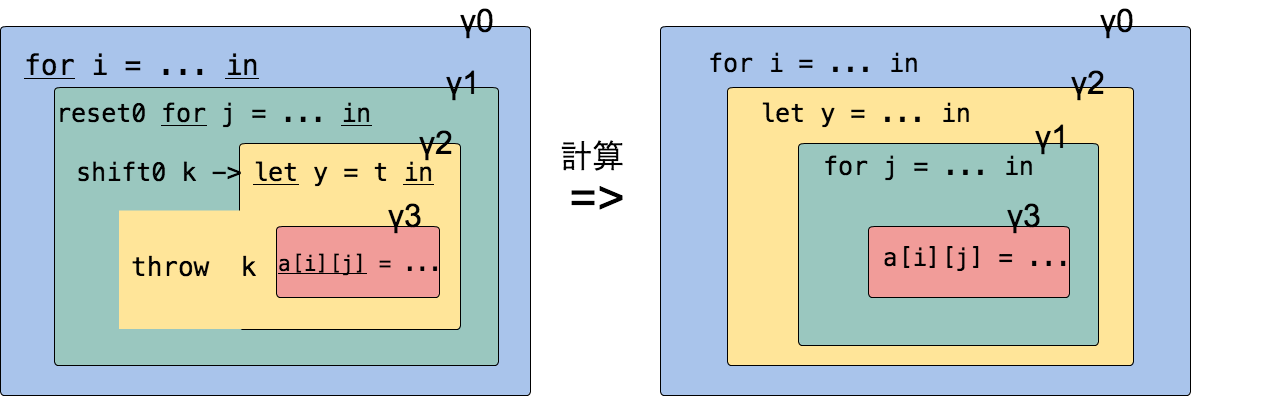
\includegraphics[clip,height=3cm]{./img/ecex_for_non_gamma.png}
\end{center}
ここで、コードレベル変数の束縛子は3つ(for式が2つとlet式が1つ)あるので、
一番外側のスコープを含め4つのスコープ(青、緑、黄、赤)が存在する。
これらに外側から順に$\gamma_0,\gamma_1,\gamma_2,\gamma_3$と名付ける。
須藤らの体系通りであれば、これらの環境識別子には、
\begin{center}
  
\includegraphics[clip,width=4cm]{./img/gamma_normal.png}
\end{center}
という順序がつくはずである。
しかし,コントロールオペレータによる計算を進めると(上記の右側の図)

\begin{center}
  
\includegraphics[clip,width=7cm]{./img/gamma.png}
\end{center}

しかし,shift0/reset0 が導入されることにより,計算の順序が



%%% Local Variables:
%%% mode: japanese-latex
%%% TeX-master: "paper"
%%% End:
